%!TEX root = ../../Main.tex
\section{Loading Virtual Machine}\label{loading-virtual-machine}

The \lstinline!expVIP! Virtual Machine (VM) allows you to analyse your
own RNA-Seq expression experiments locally.

\subsection{Requirements}\label{requirements}

The virtual machine requires:

\begin{itemize}
\itemsep1pt\parskip0pt\parsep0pt
\item
  \href{https://www.virtualbox.org}{VirtualBox}, version 5 or newer.
\item
  6GB of RAM
\item
  A 64-bit operating system running on an x86\_64 architecture. (Intel,
  AMD)
\item
  10GB of free space.
\end{itemize}

\subsection{Default data}\label{default-data}

The default values loaded in the virtual machine are available in this
\href{https://www.dropbox.com/sh/n15tpsqj92wfn8u/AABivEEUj4sRd9tG830WnSi4a?dl=0}{link}.
These correspond to the wheat data from Borrill, Ramirez-Gonzalez and
Uauy, 2015 (\emph{submitted}).

You can get a virtual machine with expVIP installed with either the
wheat data preloaded or an empty database for your analysis
\href{https://www.dropbox.com/sh/73i7ulj1hk6gdpd/AAARGuJDN0MnaZ7iLmMzSSp9a?dl=0}{here}.

\subsubsection{Available VMs}\label{available-vms}

\begin{enumerate}
\def\labelenumi{\arabic{enumi}.}
\itemsep1pt\parskip0pt\parsep0pt
\item
  \textbf{expVIPNoData.ova} This VM is ready to use, but it has no data
  on it. You can load a custom set of RNA-seq reads, transcriptome
  reference and metadata.
\item
  \textbf{expVIPwithWheatData.ova} This has all the data loaded from
  \href{http://www.wheat-expression.com}{www.wheat-expression.com}. You
  can add your own data and compare it with the values of publicly
  available experiments.
\end{enumerate}

\subsection{Setup shared folders}\label{setup-shared-folders}

To load your custom RNA-seq experiments, you have to setup a shared
folder with your input files. This shared folder will contain the data
and information required by the VM to implement expVIP and it provides
the ``connection'' between your computer and the VM. This shared folder
should include:

\begin{enumerate}
\def\labelenumi{\arabic{enumi}.}
\itemsep1pt\parskip0pt\parsep0pt
\item
  RNA-seq reads: as \lstinline!fastq! or \lstinline!fq.gz! files.
\item
  Transcriptome reference: currently only the cdna fasta file from
  ensembl is supported.
\item
  Metadata: this includes two separate files; one factor file and one
  metadata file ({[}explained here{]}
  (https://github.com/homonecloco/expvip-web/wiki/LoadingMetadata)).
\end{enumerate}

Some important information:

\begin{itemize}
\itemsep1pt\parskip0pt\parsep0pt
\item
  The shared folder must contain one sub-folder per each set of RNA-seq
  reads. So for example if you wish to analyse data from three samples,
  you will need three sub-folders (one each with the individual sample
  RNA-seq reads)
\item
  Each RNA-seq sub-folder must be named with the same accession number
  that you use in your metadata (see {[}here{]}
  (https://github.com/homonecloco/expvip-web/wiki/LoadingMetadata)).
\item
  If you wish to add your own wheat data to that previously provided in
  www.wheat-expression.com you will need to include sub-folders with
  your RNA-seq reads and then modify the metadata files:
  \lstinline!default_metadata.txt! and \lstinline!FactorOrder.tsv! which
  are provided in the \lstinline!expVIPwithWheatData.ova! or can be
  downloaded
  \href{https://www.dropbox.com/sh/n15tpsqj92wfn8u/AABivEEUj4sRd9tG830WnSi4a?dl=0}{here}.
  Additional factors and metadata can be added at the end of these files
  following similar nomenclature as that already present in the files.
\end{itemize}

\subsection{Loading the virtual
machine}\label{loading-the-virtual-machine}

Download the \lstinline!ova! virtual machine and double click it.
Virtual Box will open it. Accept the default options.

If The virtual machine is not loaded, go to the menu \lstinline!File!
and click \lstinline!Import appliance!. Open the \lstinline!.ova! you
want to use

Availabe VMs: 
\begin{description}
\item[expVIP.ova] expVIP is installed with an empty
database. This VM requires to setup your own samples. 

\item[expVIPwithWheatData.ova] expVIP is installed with the wheat
expression data, transcriptome reference and metadata. This VM allows
the inclusion of additional samples to integrate with the previously
analysed wheat data.
\end{description}

\begin{enumerate}
\def\labelenumi{\arabic{enumi}.}
\itemsep1pt\parskip0pt\parsep0pt
\item
  On the Oracle VM VirtualBox Manager select expVIP and click on the
  settings button \\ 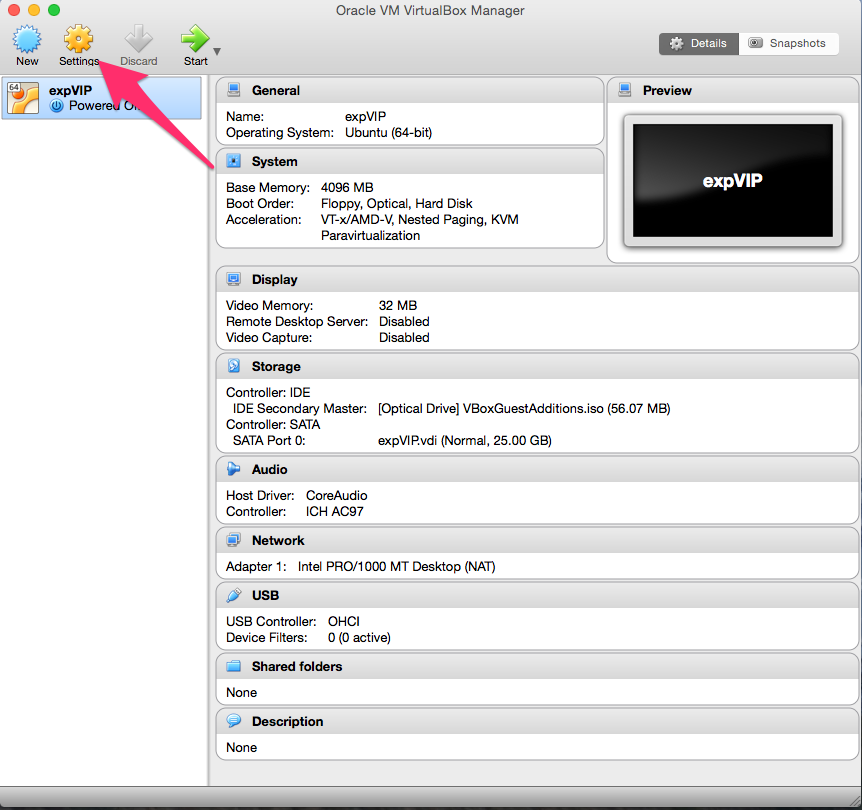
\includegraphics[width=0.75\textwidth]{expVIP/tutorial/images/Shared_Folder01.png}
\item
  Click in \lstinline!Shared folders!
  \\ 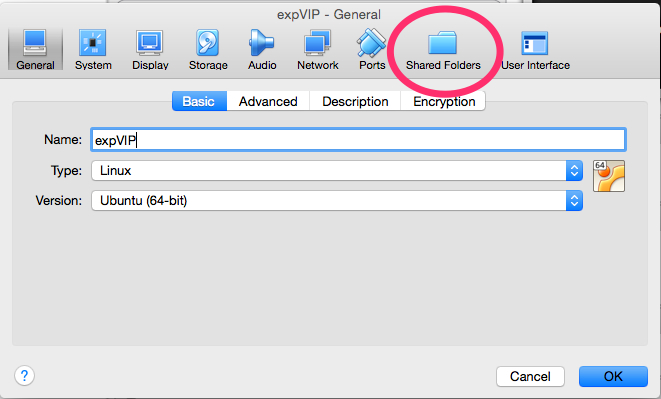
\includegraphics[width=0.75\textwidth]{expVIP/tutorial/images/Shared_Folder02.png}
\item
  Add a new folder \\ 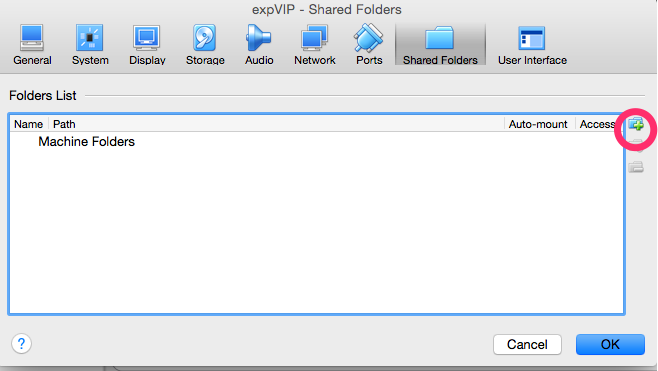
\includegraphics[width=0.75\textwidth]{expVIP/tutorial/images/Shared_Folder03.png}
\item
  Search the \lstinline!Folder path! with the experiments and the files
  with the metadata \\ 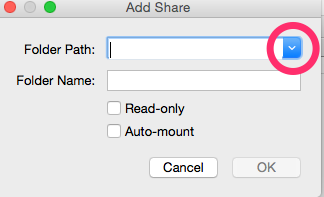
\includegraphics[width=0.75\textwidth]{expVIP/tutorial/images/Shared_Folder04.png}
  \\ 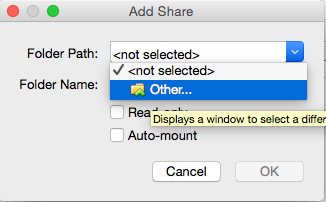
\includegraphics[width=0.75\textwidth]{expVIP/tutorial/images/Shared_Folder05.png}
\item
  Select the folder \\ 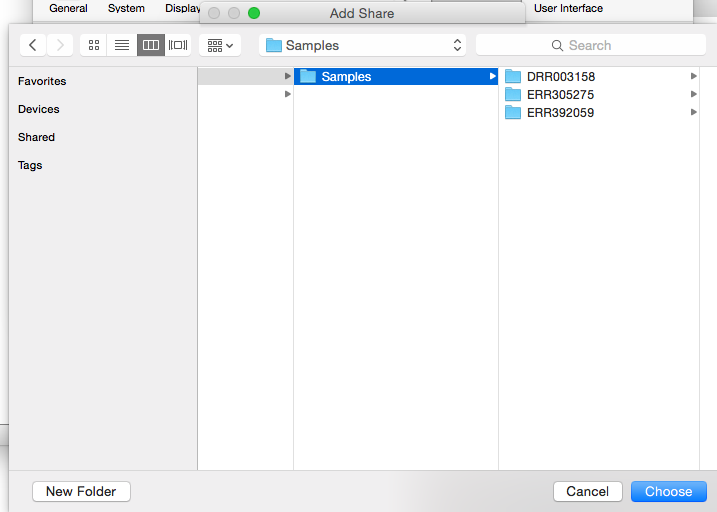
\includegraphics[width=0.75\textwidth]{expVIP/tutorial/images/Shared_Folder06.png}
\item
  Make sure that the \lstinline!Auto-mount! option is selected.
  \\ 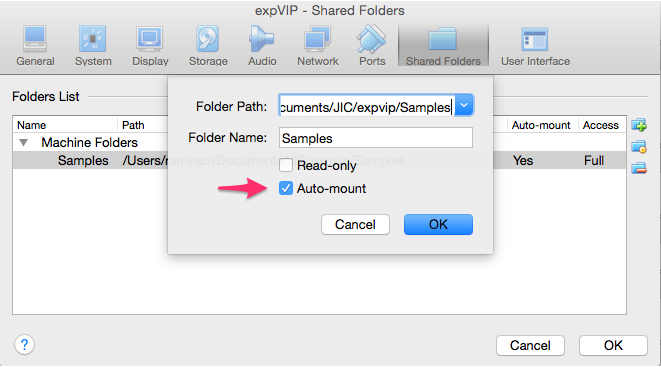
\includegraphics[width=0.75\textwidth]{expVIP/tutorial/images/Shared_Folder07.png}
\item
  Accept the settings \\ 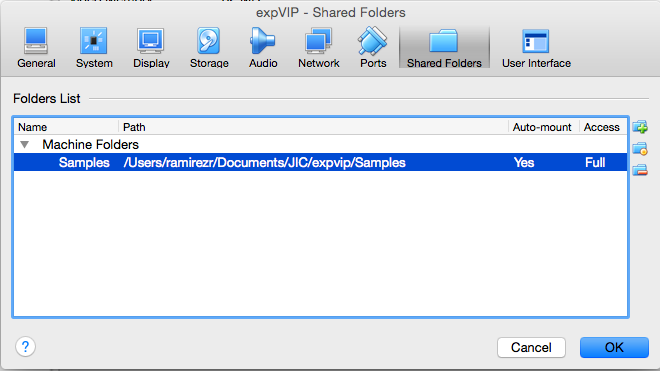
\includegraphics[width=0.75\textwidth]{expVIP/tutorial/images/Shared_Folder08.png}
\end{enumerate}

\subsection{Starting the virtual
machine}\label{starting-the-virtual-machine}

Select \lstinline!expVIP! from the VM list and press start.
\\ 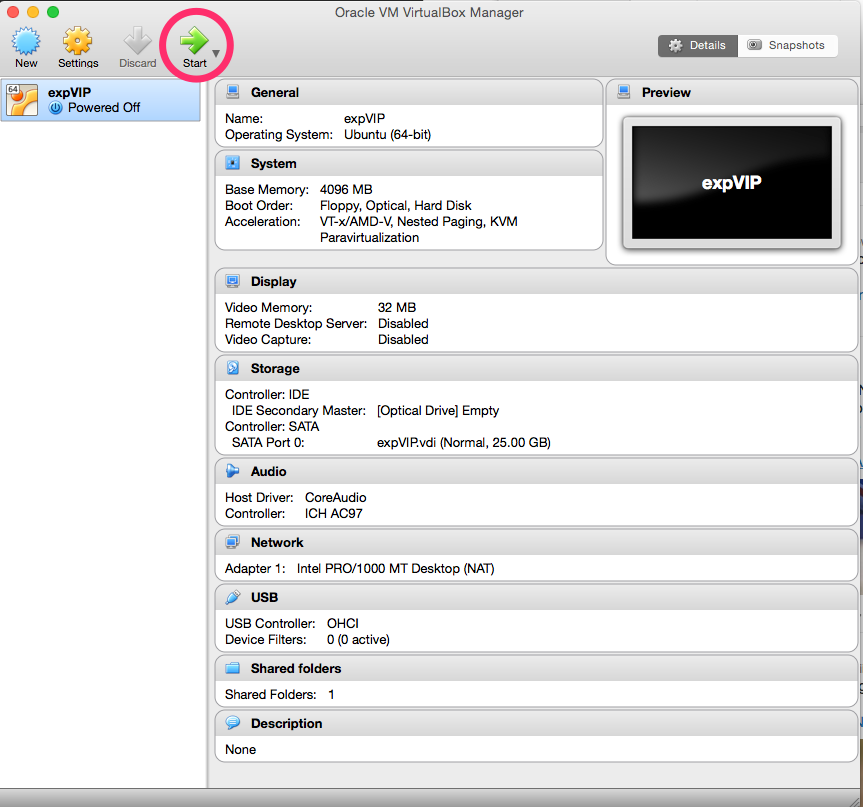
\includegraphics[width=0.75\textwidth]{expVIP/tutorial/images/StartVM01.png}

\subsection{NOTES}\label{notes}

\href{http://pachterlab.github.io/kallisto/about.html}{kallisto} is
included as part of the virtual machine and is free for non-commercial
use. However, it requires a license for commercial use. The distribution
of kallisto, with the corresponding license is included in
\lstinline!~/software/! in the VM.
